\documentclass[../mathNotesPreamble]{subfiles}

\providecommand{\relscalefact}{1.4}
\begin{document}
\relscale{\relscalefact}
  \section{2.2: Quadratic Functions: Parabolas}
  \begin{defn*}
    A \textbf{quadratic function} has the form
      \[y=f(x)=ax^2+bx+c \quad (a\neq 0)\]
      where $a$, $b$, and $c$ represent constants. A \textbf{parabola} is the shape of the graph of a quadratic function.
  \end{defn*}
  \vspace*{\stretch{1}}
  
  \begin{center}
    \begin{tikzpicture}[declare function={
      f(\x)=(\x)^2+0;
      g(\x)=-(\x)^2+0;
      h(\x)=(\x-2)^2-1;
      j(\x)=-0.5*(\x+1)^2+3;}]
      \begin{groupplot}[
        group style={group size=2 by 2, horizontal sep=20mm, vertical sep=20mm},
        grid=both, %major,minor
        grid style={line width=0.375pt, draw=gray!75},
        minor grid style={draw=gray!25},
        axis lines=center,
        axis line style={black,->},
        minor x tick num=1,
        minor y tick num=1,
        enlargelimits={value=0.05, auto},
        ticklabel style={font=\footnotesize,inner sep=0.5pt,fill=white,opacity=1.0, text opacity=1},
        every axis plot/.append style={domain=xmin:xmax, line width=0.95pt, color=lander_blue, samples=255},
        ]
        \nextgroupplot[ymin=-2.5]
          \addplot[<->] expression[domain={-3:3}]{f(x)}
            node[pos=0.92, above left, black, fill=white, opacity=0.8, text opacity=1.0, inner sep=1pt, rounded corners=2.5pt, xshift=-5pt] {$y=x^2$};
          \addplot[soldot, mark size=1.5pt] coordinates{(0,0)};
        \nextgroupplot[ymax=2.5]
          \addplot[<->] expression[domain={-3:3}]{g(x)}
            node[pos=0.91, below left, black, fill=white, opacity=0.8, text opacity=1.0, inner sep=1pt, rounded corners=2.5pt, xshift=-5pt] {$y=-x^2$};
          \addplot[soldot, mark size=1.5pt] coordinates{(0,0)};
        \nextgroupplot
          \addplot[<->] expression[domain={-1:5}]{h(x)}
            node[pos=0.925, above left, black, fill=white, opacity=0.8, text opacity=1.0, inner sep=1pt, rounded corners=2.5pt, xshift=-5pt] {$y=(x-2)^2-1$};
          \addplot[soldot, mark size=1.5pt] coordinates{(1,0)(2,{h(2)})(3,0)};
        \nextgroupplot
          \addplot[<->] expression[domain={-4:2}]{j(x)}
            node[pos=0.925, below left, black, fill=white, opacity=0.8, text opacity=1.0, inner sep=1pt, rounded corners=2.5pt, xshift=-5pt] {$y=-\frac{1}{2}(x+1)^2+3$};
          \addplot[soldot, mark size=1.5pt] coordinates{(-1-sqrt(6),0)(-1,{j(-1)})(-1+sqrt(6),0)};
      \end{groupplot}
    \end{tikzpicture}
  \end{center}
  \pagebreak
  
  \begin{defn*}
    \TabPositions{47.5mm}
    The quadratic function $y=f(x)=ax^2+bx+c$ has its \textbf{vertex} at 
      \[\parens{-\frac{b}{2a},\ f\parens{-\frac{b}{2a}}}.\]
    The optimal value occurs at the vertex of a parabola:
    \begin{itemize}
      \item A maximum if $a<0$
        \tab\tikz{\begin{axis}[axis lines=none,height=20mm]
            \addplot[<->, lander_blue] expression[domain=-1:1]{-x^2};
          \end{axis}}
      \item A minimum if $a>0$
        \tab\tikz{\begin{axis}[axis lines=none,height=20mm]
            \addplot[<->, lander_blue] expression[domain=-1:1]{x^2};
          \end{axis}}
    \end{itemize}
  \end{defn*}
  \vspace*{\baselineskip}

  \begin{center}
    \begin{tikzpicture}[declare function={
      a=-1; b=3; c=4; del=0.25;
      f(\x)=a*\x^2+b*\x+c;
      qf(\s)=(-b+\s*sqrt(b^2-4*a*c))/(2*a);
      xo=qf(1); xt=qf(-1);
      vx=-b/(2*a); vy=(b^2-4*a*c)/(4*a^2);},
      custNode/.style={
        black,
        align=center,
        inner sep=2.5pt,
        rounded corners,
        fill=white,
        opacity=0.8,
        text opacity=1.0},
      custPin/.style={
        custNode,
        pin edge={black!50}}]
      \begin{axis}[
        axis lines=center,
        axis line style={black,->},
        xmajorticks=false,
        ymajorticks=false,
        width=0.75\linewidth, height=\axisdefaultheight,
        enlargelimits={value=0.025, auto},
        every axis plot/.append style={line width=0.95pt, color=lander_blue, samples=100},
        clip=false
        ]
        \addplot[<->] expression[domain=xo-del:xt+del]{f(x)};
        \addplot[soldot] coordinates{(xo,0)(xt,0)};
        \node[custNode] (xo) at (xo,0) {};
        \node[custNode] (xt) at (xt,0) {};
        \node[custNode] (qf) at (vx,-0.275*vy) {$x=\dfrac{-b\pm\sqrt{b^2-4ac}}{2a}$};
        \draw[-, custNode, shorten >=10pt, shorten <=7.5pt] (qf) -- (xo);
        \draw[-, custNode, shorten >=10pt, shorten <=7.5pt] (qf) -- (xt);

        \addplot[soldot] coordinates{(0,c)} 
          node[above left, pin={[custPin] 120:$f(0)=c$}] {};
        \addplot[soldot] coordinates{(vx,vy)}
          node[above, pin={[custPin] $\parens{-\dfrac{b}{2a},f\parens{-\dfrac{b}{2a}}}$}, black] {};
      \end{axis}
    \end{tikzpicture}
  \end{center}
  \pagebreak


  \begin{ex*}
    Consider the function
      \[2x+\frac{x^2}{2}\]
    Is the vertex a maximum or minimum? Locate the vertex, $x$-intercepts, $y$-intercept, and then sketch the graph.
  \end{ex*}
  
  \vspace*{\stretch{1}}
  \hspace*{\stretch{1}}
  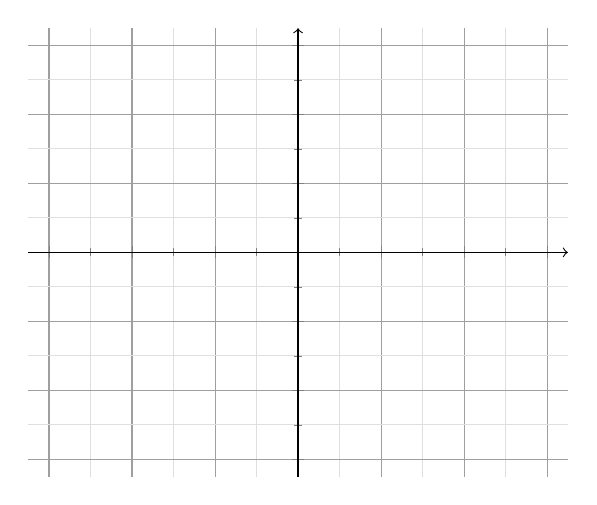
\begin{tikzpicture}
    \begin{axis}[
      grid=both, %major,minor
      grid style={line width=0.375pt, draw=gray!75},
      minor grid style={draw=gray!25},
      axis lines=center,
      axis line style={black,->},
      minor x tick num=1,
      minor y tick num=1,
      xmin=-6.5, xmax=6.5,
      ymin=-6.5, ymax=6.5,
      xticklabels={},
      yticklabels={},
      ]
    \end{axis}
  \end{tikzpicture}
  \pagebreak
  
  \begin{ex*}
    Consider the function
      \[x^2+5-4x\]
    Is the vertex a maximum or minimum? Locate the vertex, $x$-intercepts, $y$-intercept, and then sketch the graph.
  \end{ex*}
  
  \vspace*{\stretch{1}}
  \hspace*{\stretch{1}}
  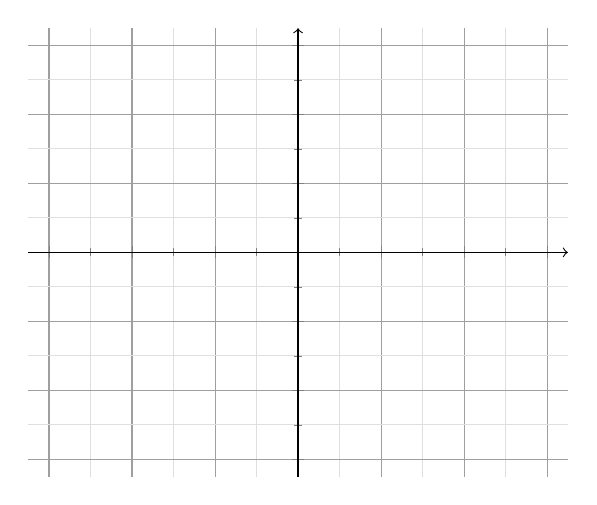
\begin{tikzpicture}
    \begin{axis}[
      grid=both, %major,minor
      grid style={line width=0.375pt, draw=gray!75},
      minor grid style={draw=gray!25},
      axis lines=center,
      axis line style={black,->},
      minor x tick num=1,
      minor y tick num=1,
      xmin=-6.5, xmax=6.5,
      ymin=-6.5, ymax=6.5,
      xticklabels={},
      yticklabels={},
      ]
    \end{axis}
  \end{tikzpicture}
  \pagebreak
  
  \begin{ex*}
    Ace Cruises offers a sunset cruise to a group of $50$ people for a price of $\$30$ per person, but it reduces the price per person by $\$0.50$ for each additional person above $50$. Find the revenue function. What price maximizes the revenue? What is this maximal value?
  \end{ex*}

  \pagebreak
\end{document}
